\documentclass[fleqn]{scrartcl}
\usepackage[T1]{fontenc}
\usepackage[utf8x]{inputenc}
\usepackage{scrpage2}
\usepackage{paralist}
\usepackage{titling}
\usepackage{tabularx}
\usepackage{amsmath}
\usepackage{amsfonts}
\usepackage{amssymb}
\usepackage{mathtools}
\usepackage{ucs}
\usepackage[shortlabels]{enumitem}
\usepackage{graphicx}
\usepackage{listings}
\usepackage{tikz}
\usepackage{xcolor}

\definecolor{deepblue}{rgb}{0,0,0.5}
\definecolor{deepred}{rgb}{0.6,0,0}
\definecolor{deepgreen}{rgb}{0,0.5,0}

\lstset{
language=Python,
breaklines=true,
otherkeywords={self,nonlocal},             % Add keywords here
keywordstyle=\bfseries\color{orange},
emph={__init__},          % Custom highlighting
emphstyle=\color{deepred},    % Custom highlighting style
stringstyle=\color{deepgreen},
frame=tb,                         % Any extra options here
showstringspaces=false,            %
numbers = left
}

\pagestyle{scrheadings}
\clearscrheadfoot
\cfoot[\pagemark]{\pagemark}
\author{Tom Schmidt\\216204224 \and Stefan Poggenberg\\218100161 \and Samuel Schöpa\\216203821 \and Bjarne Hiller\\216203851}
\title{KI HA 2}
\date{22. Juni 2018}

\begin{document}
\maketitle

\section{Anmerkung zu CSP mit Heuristik}
\textbf{Grundlegende Idee}
\begin{itemize}
	\item erstelle Adjazentmatrix für den Graph
 	\item streiche in jedem Schritt die Zeile und Spalte aus der Matrix, mit den wenigsten Nachbarn \\
 	falls mehrere Einträge gleicher Länge auftauchen, wähle zufälligen Eintrag
	\item sollte mit dem letztgestrichenden Eintrag keine Lösung möglich sein, füge diesen wieder in die Adjazentmatrix ein (beachte dabei natürlich die veränderten Nachbarschaften, \\
durch vorherige Streichungen)	 
\end{itemize}
\textbf{Testergebnisse nach 10 runs}
\begin{itemize}
	\item \textit{mit Heuristik: } 46, 49, 37, 16, 28, 48, 43, 44, 42, 53  backtrackcsp-Calls
	\item \textit{ohne Heuristik: } konstant 9 backtrackcsp-Calls
	\item \textit{Abschließende Frage: } Ist die Heuristik nun schlechter als die Lösung, ohne Heuristik?
\end{itemize}

\section{Schiebepuzzles als Planungsproblem}
\subsection{3}
\begin{figure}[h!]
  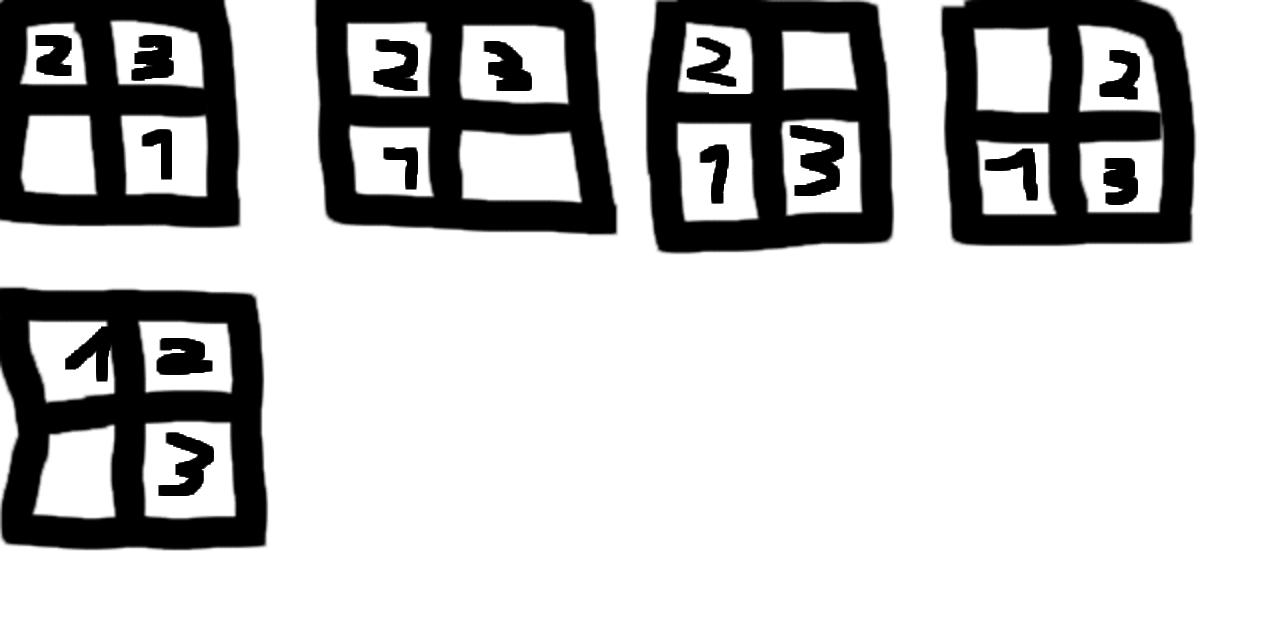
\includegraphics[width=\linewidth]{a2/3.PNG}
\end{figure}
\subsection{4}
  at(tile, position): Ist an gegebener Position gegebenes tile? \\
  empty(position): Ist auf der Position kein tile? \\
  neighbor(position, position): Liegen gegebene Positionen nebeneinander? \\
  move(tile, position): Bewege gegebenes tile auf gegebene Position. \\
\subsection{5}
\subsubsection{domain.pddl}
\lstinputlisting[firstline=1, lastline=25]{a2/domain.pddl}
\subsubsection{problem.pddl}
\lstinputlisting[firstline=1, lastline=32]{a2/problem.pddl}

\section{Bayerische Filter}
\begin{figure} [h!]
 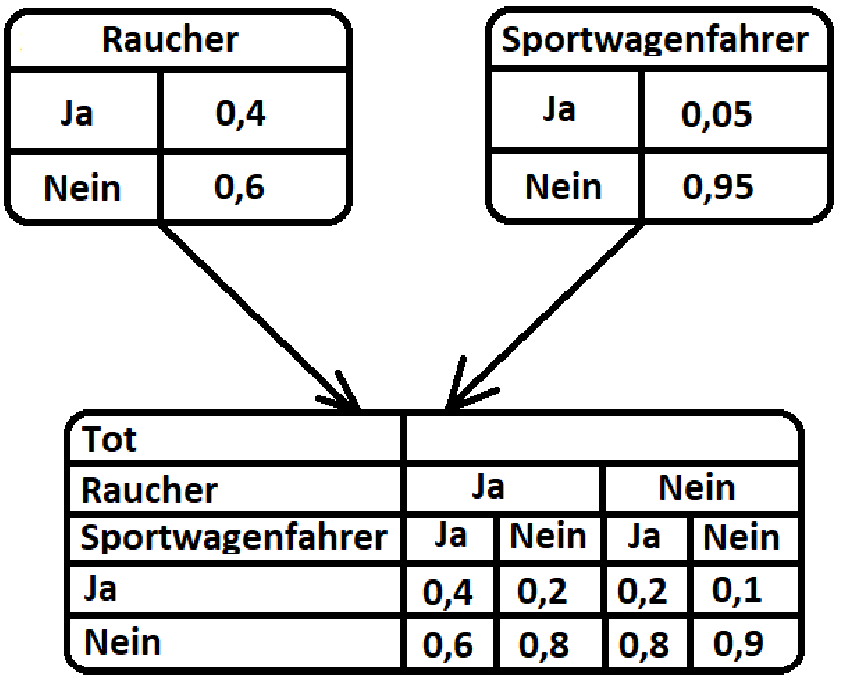
\includegraphics [width = \linewidth] {a2/Bayessches_Netz.PNG}
\end{figure}


\end{document}
